%!TEX encoding = UTF-8 Unicode
\vfill
\pagebreak
\section{Related Work}
\label{sec:RelatedWork}
% Show what you read Start by presenting the structure of component. Show each
% item in a different section. Which works are known as relevant in this area
% Each section should end with a comparative evaluation. End each chapter with a
% synthesis, a table about various solutions, which features are interesting,
% which we want. Finnish sections with a work summary on a single sentence.

The solution proposed in this document leverages knowledge obtained from
studying several concepts and systems from the current state-of-the-art. In this
section an overview of those concepts and systems will be given, stating for
each of them their advantages and disadvantages.\\
This section is structured as follows. Section \ref{sec:Computingparadigms} presents different methods to push intelligence and computing power closer to the source of the data and why this work adopted fog computing for this purpose. Section \ref{sec:Mobility} presents
mobility-aware systems xxx. Section \ref{sec:Dataplacement} xxx. \ref{sec:Migration} xxx. \ref{sec:Multiobjective} xxx. Section \ref{sec:Toolkits} xxx.

\subsection{Computing paradigms}
\label{sec:Computingparadigms}
In what concerns about standardizing fog computing, there is a lack of unanimity. As aforementioned, fog has been variously termed as cloudlets, edge computing, etc. Different research teams are proposing many independent definitions of fog (and fog-related computing paradigms). As there is a research gap in the definitions and standards for fog computing, this work follows the definitions that Ashkan Yousefpour et al. \cite{yousefpour2018all} proposed. Below, are described some of the paradigms that were raised in order to bring cloud closer to the end devices, as well as their pros and cons. As a conclusion we show why fog computing is the natural platform for IoT.

\subsubsection{Mobile computing}\label{subsec:MC}
Mobile/nomadic computing (MC) is characterized by the processing being performed by mobile devices (e.g., laptops, tablets, or mobile phones). It raises to overcome the inherent limitations of environments where connectivity is sparse or intermittent and where there is low computing power. As this model only uses mobile devices to provide services to clients, there is no need for extra hardware, once they already have communication modules such as Bluetooth, WiFi, ZigBee, etc. As already mentioned, mobile devices have evolved in recent years, however their resources are more restricted, compared to fog and cloud. This computing paradigm has the advantage of being characterized by a distributed architecture, once mobile machines do not need a centralized location to operate. The disadvantages of MC are mainly due to their hardware nature (i.e. low resources, balancing between autonomy and the dependency of other mobile devices; characteristic that prevails in all distributed architectures) and the need of mobile clients to efficiently adapt to changing environments \cite{satyanarayanan1996fundamental}. MC alone may not be able to meet the requirements of some applications. On the one hand it is limited due to autonomy constraints and in the order hand low computational power and low storage capacity further restricts the applications where this paradigm is feasible. For instance it is unsuitable for applications that require low-latency or that generates large amounts of data that needs to be stored or processed. Nonetheless, MC can use both fog and cloud computing to enhance its capacities, not being restricted to a local network; expanding the scope of mobile computing and the number of applications where it can be used.\vfill\pagebreak

\subsubsection{Mobile Cloud Computing}
Cloud and fog computing, as mentioned in \ref{subsec:MC}, are key elements for validate the importance of MC. This interaction between them results in a new paradigm, called mobile cloud computing (MCC). MCC, differs from MC in a sence that mobile applications can be partitioned at runtime so that computationally intensive components of the application can be handled through adaptive offloading \cite{shiraz2013review}, from mobile devices to the cloud. This characteristic increases the autonomy of mobile devices (i.e battery lifetime), as both the data storage and data processing occur outside of the mobile device. Also, it enables a much broader range of mobile subscribers, rather then the previous laptops, tablets, or mobile phones. Opposed to resource-constrained in MC, MCC has high availability of computing resources, scaling the type of applications where it is possible to use, for instance, augmented reality applications. Unlike MC, MCC relies on cloud-based services, where its access is done through the network core by WAN connection, which means that applications running on these platforms require connection to the Internet all the time. On the one hand, both MCC an MC suffer from the intrinsic characteristics of mobility, such as frequent variations of network conditions, intensified under rapid mobility patterns. On the other hand, in MCC, even if the mobile devices remain fixed, it suffers from the inherent disadvantage of using cloud-based services (i.e. communication latency), which makes it unsuitable for some delay-sensitive applications.

\subsubsection{Mobile ad hoc Cloud Computing}
In some scenarios there exists lack of infrastructure or a centralized cloud, so implement a network based on MCC may not always be suitable. To overcome dependence on an infrastructure, raises mobile ad hoc cloud computing (MACC). It consists on a set of mobile nodes that form a dynamic and temporary network through routing and transport protocols. These nodes are composed by mobile ad hoc devices which may continuously join or leave the network. In order to counteract the, aforementioned, characteristics inherent to this type of networks, and unlike MC, a set of ad hoc devices may form a local cloud that can be used in the network for purposes of storage and computation. As mobile ad hoc networks (MANET), it can play a big part in use cases such as disaster recovery, car-to-car communication, factory floor automation, unmanned vehicular systems, etc. Although it does not rely in external cloud-based services as MCC does, which mitigates the latency problem, it shares some of the limitations inherent to MC and ad hoc networks such as the power consumption constraints. Moreover, the formed local cloud may still be computationally weak and as both network and cloud are dynamic it is more challenging to achieve an optimal performance. For instance, as there is no infrastructure, mobile devices are also responsible for routing traffic among themselves.

\subsubsection{Edge Computing}
Edge computing (EC), enhances their capabilities (i.e. management, storage, and processing power) by connected devices at the edge of the network. Edge computing is located in the local IoT network, being ideally at one hop away from the Iot device and at most located few hop away. Open Edge Computing defines edge computing as computation paradigm that provides small data centers (edge nodes) in close proximity to the users, enabling a dramatic improvement in customer experience through low latency interaction with compute and storage resources just one hop away from the user \cite{OpenEdge73:online}. As in EC the connected devices do not have to wait for a centralized platform to provide a requested service, nor are so limited in terms of resources as in the traditional MC, their service availability is relatively high. Nonetheless EC has some drawbacks. As latency, in this context, is composed by three components: data sending time, processing time and result receiving time, even though the communication latency is negligible, processing time may not be. This computing paradigm only uses edge devices, and their computation and storage power may be poor (e.g., routers, switches). Consequently, this processing latency may still be too high for some applications with low latency requirements.\\
\noindent\tab OpenFog Consortium states that fog computing is often erroneously called edge computing, but there are key differences \cite{OpenFog0208}. Although they have similar concepts, edge computing tends to be limited to the edge devices (i.e. located in the IoT node network), excluding the cloud from its architecture. Whereas, fog computing is hierarchical and unlike EC, it is not limited a local network, but instead it provides services anywhere from cloud to things. It is worth noting that the term edge used by the telecommunications industry usually refers to 4G/5G base stations, radio access networks (RANs), and internet service provider (ISP) access/edge networks. Yet, the term edge that is recently used in the IoT landscape refers to the local network where sensors and IoT devices are located \cite{yousefpour2018all}.

%muita coisa copiada, tentar reescrever
\subsubsection{Multi-access Edge Computing}
Analogously, MCC is an extension of MC through cloud computing, as multi-access edge computing (MEC) is an extension of MC through EC. ETSI defines MEC as computation paradigm that offers application developers and content providers cloud-computing capabilities and an IT service environment at the edge of the network. This environment is characterized by ultra-low latency and high bandwidth as well as real-time access to radio network, information that can be leveraged by applications \cite{ETSIMult81:online}. In MEC, operators can open their RAN edge to authorized third parties, allowing them to deploy applications and services towards mobile subscribers through 4G/5G base stations. The first approach to the edge of a network meant the edge of a mobile network, hence the name mobile edge computing. As MEC research progressed, was noticed that the term leaves out several access points that may also construct the edge of a network. Thus, prompted the change from mobile edge computing to multi-access computing in order to reflect that the edge is not solely based on mobile networks \cite{MobileEd74:online}. Now it include a broader range of applications beyond mobile device-specific tasks, such as video analytics, connected vehicles, health monitoring, augmented reality, etc.\\
MEC supports low-latency applications once it benefits from real-time radio and network information. Similar to edge computing, MEC can operate with little to no Internet connectivity and use small-scale data centers with virtualization capacity to provide services. Unlike EC, MEC establishes connectivity through a WAN, WiFi, and cellular connections, whereas edge computing generally can establish any form of connectivity (e.g., LAN, WiFi, cellular). MCC focuses on the relationship between cloud service users (on mobile devices) and cloud service providers, whereas research in MEC focuses on (RAN-based) network infrastructure providers. MEC allows edge computing to be accessible to a wide range of mobile devices with reduced latency and more efficient mobile core networks \cite{taleb2017multi}.SDN allows for virtual networking devices to be easily managed through software APIs \cite{kadiyala2017inter}, and NFV allows for reduced deployment times for networking services through virtualized infrastructure. MEC is expected to benefit significantly from the up-and-coming 5G platform as it allows for lower latency and higher bandwidth among mobile devices, and it supports a wide range of mobile devices with finer granularity.

\subsubsection{Cloudlet Computing}
Cloudlet computing is another direction in mobile computing that aims to bring cloud closer to end devices through the use of cloudlets. M. Satyanarayanan et al. states that a cloudlet is a trusted, resource-rich computer or cluster of computers that’s well-connected to the Internet and available for use by nearby mobile devices \cite{satyanarayanan2009case}. Cloudlet is, as the name suggests, a smaller sized clouds with lower computational capacity. It can be seen as a ``data center in a box'', where mobile users can exploit their virtual machines (VM) to rapidly instantiate customized-service software in a thin client fashion. This way, it is possible to offload computation from mobile devices to VM-based cloudlets located on the network edge. Through those VMs, cloudlets are capable of providing resources to end devices in real time over a WLAN network. The relatively low hardware footprint, results in moderate computing resources, but lower latency, energy consumption and higher bandwidth compared to cloud computing. The characteristics of this computing paradigm make possible to handle applications with low-latency requirements, supporting real-time IoT applications.
Y Jararweh et al. \cite{jararweh2013resource} propose an architecture mobile-cloudlet-cloud, where they present three reasons which indicate that even though cloudlets are computationally powerful, they still need a connection to the cloud and its services: (1) Heavy non real time jobs might process in the enterprise cloud whiles the real time ones processed by the cloudlet, (2) Accessing a file stored in the Enterprise Cloud, (3) Accessing some services that are not available inside the Cloudlet. Although cloudlet computing fits well with the mobile-cloudlet-cloud architecture, fog computing offers a more generic alternative that natively supports large amounts of traffic, and allows resources to be anywhere along the thing-to-cloud continuum.

%muita coisa copiada, tentar reescrever
\subsubsection{Mist Computing}
Mist computing emerges to push IoT analytics to the extreme edge. This computing paradigm is an even more dispersed version of fog. That means locating analytics tools not just in the core and edge, but at the ``extreme edge'' - actually in many of the devices (the IoT devices themselves; the sensor and actuators) \cite{Ciscopus95:online}. It has been proposed with future self-aware and autonomic systems in mind \cite{preden2015benefits}. Therefore, mist computing can be seen as the first computing location in the IoT-fog-cloud continuum. Mist computing extends compute, storage, and networking across the fog through the things. This decreases latency and increases subsystems’ autonomy. The challenge with implementing mist computing systems lies in the complexity and interactions of the resulting network, which must be managed by the devices themselves as central management of such systems is not feasible.

\subsubsection{Fog computing}
Fog computing bridges the gap between the cloud and IoT devices by enabling computing, storage, networking, and data management on the network nodes within the close vicinity of IoT devices. OpenFog Consortium \cite{WhatIsFo95:online} defines fog computing as ``a horizontal system-level architecture that distributes computing, storage, control and networking functions closer to the users along a cloud-to-thing continuum.'' The decentralized nature of fog computing allows devices to either serve as fog computing nodes themselves (e.g. a car acts as a fog node for on-board sensors) or use fog resources as the clients of the fog (end device). Compared to the cloud, fog computing offers moderate computing capacity and low power consumption. Clouds are composed by large datacenters whereas fog uses small servers, routers, switches, gateways, set-top boxes or access-points (AP). Fog has lower hardware footprint, so it can be closer to the end devices. Fog computing can be accessed through connected devices from the edge of the network to the network core, whereas cloud computing must be accessed through the network core. Moreover, continuous Internet connectivity is not essential for the fog-based services to work. That is, the services can work independently with low or no Internet connectivity and send necessary updates to the cloud whenever the connection is available. Cloud computing, on the other hand, requires devices to be connected when the cloud service is in progress. There are clear differences and tradeoffs between cloud and fog computing, and one might ask which one to choose. However, fog and cloud complement each other; one cannot replace the need of the other. By coupling cloud and fog computing, the services that connected devices use can be optimized even further.

\subsubsection{Other Similar Computing Paradigms}
\begin{itemize}
	\item \textbf{Micro Data Center} (MDC) - Cloudlet são por vezes referidas
	como MDC. Um MDC pode ser um edge node ou uma cloudlet que é implementada
	entre os dispositivos IoT e a cloud.
	\item \textbf{Cloud of Things} (CoT) - Parecido a mist computing, no entanto
	em mist a computação é feita nos dispositivos IoT e não necessariamente numa
	cloud de pooled resources. Em CoT, a computação é feita sobre a cloud que é
	formada por pooled resources de IoT devices.
	\item \textbf{Edge Cloud} - Quando falamos de cloud computing, falamos de
	"core" ou "distant" clouds que estão distantes do end users que são
	responsáveis pela computação "pesada". Ao contrário, "edge" clouds são mais
	pequenas e estão mais próximas. Edge cloud é parecido a edge computing. Edge
	cloud extende capacidades da cloud na edge aproveitando os compute nodes
	(user ou operator-contributed) na edge da rede. À semelhança do fog, em edge
	clouds a habilidade de correr uma aplicação numa forma coordenada tanto na
	edge com na cloud é prevista. Edge clouds são nós na edge como micro data
	centers, cloudlets, e MEC.
\end{itemize}

\subsubsection{Concluding Remarks}
As the above mentioned, there are some other similar computing paradigms such as follow me cloud (FMC), follow me edge (FME), Follow Me edge-Cloud (FMeC), etc. However, this state-of-the-art had as objective to investigate the most treated ones in the literature. The purpose was to understand their characteristics and identify where to tackle the current limitations of delay sensitive IoT applications and consequently their deployment.

The previous discussion about fog computing and related paradigms demonstrate the importance of understanding the characteristics of these platforms in the changing IT landscape. As demonstrated by the strength and weaknesses attributed to these computing paradigms, some paradigms may be better suited for a particular
use case than others. Even so, fog computing is suited for a large number of use cases in the current landscape of IoT and connected devices. The versatility of fog computing makes it suitable for many cases of data-driven computing and low-latency applications, even though it may not be suitable for a few extreme applications, such as disaster zones or sparse network topologies where ad hoc computing (e.g., MACC) or extreme edge clouds (e.g., mist, CoT) may be a better fit. Nonetheless, fog computing is considered a more general form of computing when compared to other similar paradigms (e.g., EC, MEC, cloudlet), because of its comprehensive definition scope, generality, and extensive presence along the thing-to-cloud continuum. Tables 2 and 3 summarize these characteristics. Fog computing offers a bright future for an open-standards environment of connected devices, as it is evident by IEEE Standard’s adoption of OpenFog Reference Architecture [69]. There does not yet exist a globally unanimous distinction between fog computing and related computing paradigms, such as edge computing, mist computing, and cloudlets across researchers and industries, as shown in the previous sections of this paper. We attempt in this survey paper to clarify the distinctions between fog computing and the related computing paradigms. A comparison of the underlying infrastructure of fog computing and its related computing paradigms from the networking perspective is shown in Fig. 7. In the rest of this paper, we will mainly survey and discuss the recent literature on fog computing, but mention the studies on other related computing paradigms that could be easily extended or directly applied in fog.

\begin{figure}
	\centering
	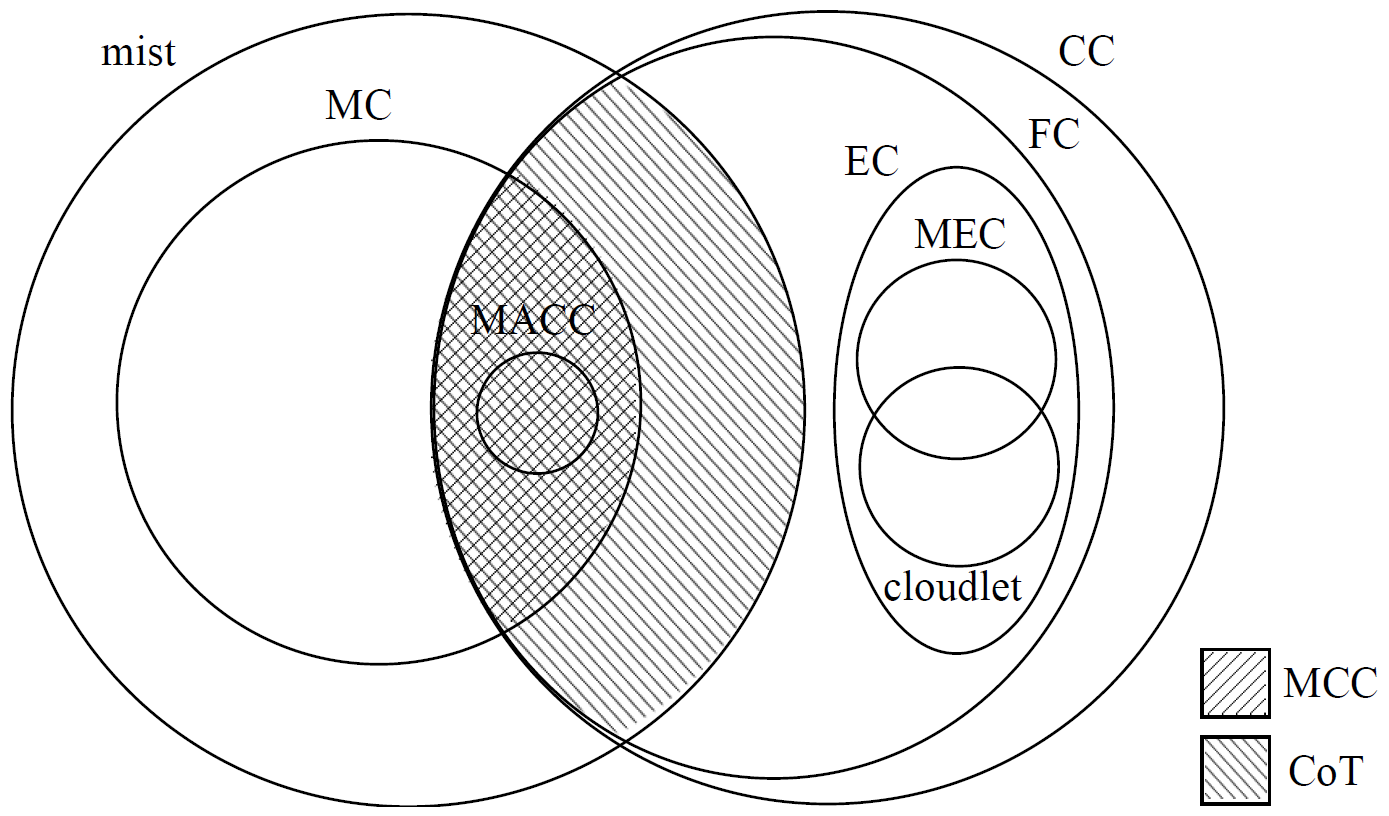
\includegraphics[width=90mm]{images/computing_paradigms}
	\caption{A classification of scope of fog computing and its related computing paradigms.}
	\label{architecture}
\end{figure}

\subsection{Mobile Fog Computing}
\label{sec:Mobility}
Mobile Fog Computing is the ability to provide mobility support for both IoT and
Fog nodes. This means that users holding end devices, can outsource the
allocation and management of resources to the fog infrastructure, where both iot
and fog nodes are able to move, ensuring that QoS requirements of the IoT
applications are met.\\
Several studies were already done in order to provide mobile support for IoT
devices, however, the purpose of this study is to support mobile Fog Computing,
once in smart cities, fog nodes cloud be anything from things to the cloud.

This distributed middle tier, in a 3-tier architecture, things-fog-cloud, can
use as fog nodes any physical device that has facilities or infrastructures that
can provide resources and visualization capabilities.  This, may include movable
fog nodes, such as cars, buses, unmanned aerial vehicles (UAVs), etc.\\
In this field there are already some early efforts

falar dos vários exemplos que o stor gosou. no final referir que a cloud utiliza VMs para .... (wikipedia), e que fog para além disto utiliza as VMs para sportar a mobilidade. Falar das possibilidades VM num todo ou floglets...........

%\noindent\tab Fog computing will be crucial in a diversity of scenarios. For
%instance, heterogeneous sensory nodes (e.g., sensors, controllers, actuators)
%on a self-driving vehicle, are estimated to generate about 1GB data per second
%\cite{angelica2013google}. As the number of features grow, the data deluge
%grows out of control. Moreover, these types of systems, where people's lives
%depends on it, are hard real-time what means that it is absolutely imperative
%that all deadlines are met. Offloading tasks to fog nodes will be the best
%solution, once a big effort in mobility support has been done through the
%migration of VMs using cloudlets \cite{lopes2017myifogsim}. Also, in this
%context, Puliafito et al. address three types of applications where fog is
%required, namely, citizen's healthcare, drones for smart urban surveillance and
%tourists as time travellers \cite{puliafito2017fog}, addressing the needs of
%low latency and mobility support.\\


%\subsubsection{Mobile IoT nodes} \label{subsec:MobileIoTnodes}

%\subsubsection{Mobile Fog nodes} \label{subsec:MobileFognodes}

%\subsubsection{Mobile Fog computing} \label{subsec:MobilityFog}

\subsection{Data placement}
\label{sec:Dataplacement}

%\subsubsection{Virtual Objects} \label{subsec:VirtualObjects}

%\subsubsection{Virtual Machines} \label{subsec:VirtualMachines}

\subsection{Migration Optimization}
\label{sec:Migration}

\subsection{Multi-objective}
\label{sec:Multiobjective}
QoS, QoE, Cost, Energy, Handover, Mobility, Bandwidth
\subsection{Toolkits}
\label{sec:Toolkits}

\vfill\pagebreak
